\documentclass[9pt, aspectratio=169]{beamer}

\usetheme{metropolis}
\usepackage{appendixnumberbeamer}

\usepackage{booktabs}
\usepackage[scale=2]{ccicons}

\usepackage{pgfplots}
\usepgfplotslibrary{dateplot}

\usepackage{xspace}
\newcommand{\themename}{\textbf{\textsc{metropolis}}\xspace}

\usepackage[brazilian,hyperpageref]{backref}	 % Paginas com as citações na bibl
\usepackage[alf]{abntex2cite}	% Citações padrão ABNT

%Tabelas
\usepackage{tabularx}
\usepackage{adjustbox}
\usepackage{pgfplotstable}

% Equações
\newcommand{\dmc}{\(DMC_x^2\) }
\newcommand{\pdcca}{\({\rho}_{DCCA}\) }
\newcommand{\fdfa}{\(F_{DFA}\) }

% Dados da apresentação

\title{\dmc e aprendizado de máquina aplicados à análise de séries temporais de dados meteorológicos}
\subtitle{Apresentação do andamento da pesquisa}
%\date{\today}
\date{15/05/2023}
\author{Discente: Fernando Ferraz Ribeiro \\Orientador: Prof. Dr.Gilney Figueira Zebende \\Co-orientador: Prof. Dr. Juan Alberto Leyva Cruz}



\institute{UEFS PPGM - Feira de Santana, BA}

\titlegraphic{\hfill
\includegraphics[height=1.0cm]{../Figures/Logo_Uefs.jpg}
\includegraphics[height=1.0cm]{../Figures/logoPPGM-UEFS.png}}

\begin{document}

\maketitle

\begin{frame}{Sumário}
  \setbeamertemplate{section in toc}[sections numbered]
  \tableofcontents[hideallsubsections]
\end{frame}

\section{Introdução}

\begin{frame}[fragile]{Sistemas Complexos}

  Este conjunto amplo de fenômenos é comumente identificado e agrupado por algumas de suas características: são formados pela contribuição de um conjunto (geralmente grande) de componentes (muitas vezes simples) que, interagindo, estruturam-se de forma auto-organizada, gerando resultados inesperados, que não podem ser previstos pelos estudos estatísticos e/ou matemáticos tradicionais dos elementos formadores do sistema.

\end{frame}

\begin{frame}
  \frametitle{Reconhecimento}

  Em 2021, a Academia Real das Ciências da Suécia concedeu metade do Prêmio Nobel de Física para Syukuro Manabe e Klaus Hasselmann, cujos estudos apresentam modelos complexos para a análise do clima. Em particular apontam uma correlação entre as emissões de dióxido de carbono e as mudanças climáticas.  

\end{frame}

\begin{frame}
  \frametitle{Sistemas Complexos e Ciência de Dados}

  Muitos fenômenos complexos são investigados pela análise de grandes conjuntos de dados. É notável a velocidade e quantidade de dados que são gerados e armazenados pela humanidade atualmente. A aquisição, manipulação, gestão, armazenamento e criação de valor a partir de dados, através de ambientes computacionais, tem-se apresentado como um novo paradigma tecnológico. Um campo do conhecimento que recebeu a denominação de Ciência de Dados, conceito que envelopa alguns termos frequentemente associados à inovação científica, técnica e social como \emph{Big Data}, mineração de dados, \emph{Business Intelligence} internet das coisas, inteligência artificial e aprendizado de máquina(AM), dentre outros \cite[p. 12-13]{EMCdata2015}.

\end{frame}

\begin{frame}
  \frametitle{Séries Temporais}

  As séries temporais são definidas como um conjunto de observações (numéricas ou categóricas) ordenado no tempo.  Embora muitos dos dados que descrevem as dinâmicas espaciais podem ser registrados na forma de sérias temporais (abastecimento de água nas tubulações, consumo de energia elétrica nos imóveis, fluxos de pessoas e veículos pela cidade, casos de uma doença por dia, etc.), contudo as técnicas de medição de correlações, bem como a devida exploração destas para inferir novos conhecimentos, permanecem como perguntas abertas em muitas sub-áreas das ciências ambientais\cite{Bermudez-Edo2018}.

\end{frame}

\begin{frame}{Proposta}

  Esta pesquisa propõe-se um estudo de dois conjuntos de variáveis meteorológicas, utilizando o \dmc como ferramenta de medição das correlações entre múltiplas variáveis. Após a avaliação dos resultados destes estudos, propõe-se a criação de um modelo preditivo utilizando ferramentas de AM e o \dmc.
  
\end{frame}

\begin{frame}{Objetivo Principal}

  O objetivo principal desta pesquisa é: investigar as correlações entre as variáveis meteorológicas de diferentes localidades através do coeficiente \dmc e utilizar o conhecimento destas correlações para alimentar um modelo preditivo de condições meteorológicas.

\end{frame}

\begin{frame}{Objetivos Gerais}

  \begin{enumerate}
    \label{enum:obj_espec}
    \item Implementar um algoritmo computacional geral para calcular o \dmc para qualquer número de séries temporais.
    \item Analisar um conjunto de dados climáticos contendo medições meteorológicas de todas as capitais brasileiras.
    \item Analisar um conjunto de dados meteorológicos sobre radiação solar com estações locadas em diversas partes do globo.
    \item Desenvolver e implementar um algoritmo de predição baseado em aprendizado de máquina e redes neurais artificias agregados com o coeficiente \dmc.
\end{enumerate}

\end{frame}

\begin{frame}
  \frametitle{Premissas}

  \begin{enumerate}
    \label{enum:premissas}
    \item Os fenômenos climáticos estão relacionados de forma complexa. Por exemplo: massas de ar percorrem distâncias na atmosfera e influenciam uma série de variáveis climáticas nas localidades por onde passam, mas que também são influenciadas, em seu percurso ou sua dissolução pelas mesmas variáveis.
    \item O \dmc, pelas características de análise do método, pode ajudar a entender estas correlações.
    \item O \dmc~é uma generalização do método \pdcca~para múltiplas séries temporais.
	\item O \pdcca, em determinadas condições testadas, apresentou resultados mais interessantes (como melhor descrição dos fenômenos) que os apresentados pelo coeficiente de Pearson quando aplicado à séries temporais~\cite{Wang2013}. 
\end{enumerate}

\end{frame}

\begin{frame}
  \frametitle{Questões}

  \begin{enumerate}
    \label{enum:quest}

    \item É possível estabelecer e medir correlações entre variáveis meteorológicas de uma determinada localidade e um conjunto de outras localidades?

    \item Em caso de resposta positiva, seria possível utilizar essas correlações para melhorar modelos meteorológicos preditivos?
\end{enumerate}

\end{frame}

\begin{frame}
  \frametitle{Hipóteses}

  \begin{enumerate}
    \item Um método baseado no \dmc~seria um ferramental importante no estudo de correlações de variáveis climáticas envolvendo um grande número de localidades.
	\item É possível criar uma modelo preditivo para séries temporais de aprendizado de Máquina eficiente baseado no \dmc.
\end{enumerate}

\end{frame}


\section{Aspectos Metodológicos}

\begin{frame}
  \frametitle{Fontes de dados}

Instituto Nacional de Meteorologia (INMET) \url{https://portal.inmet.gov.br/}. Do massivo conjunto de dados disponível, foram baixados apenas os registros das capitais.

Baseline Surface Radiation Network (BSRN) \url{https://bsrn.awi.de/}. Uma rede de medições meteorológicas de alta precisão com estações filiadas no mundo inteiro. 

\end{frame}

\begin{frame}
  \frametitle{Metodologia}

  Com os dois conjuntos de dados organizados, para cada uma das análises seguiremos as seguintes etapas.

\begin{enumerate}
    \item Análise exploratória dos dados e identificação das necessidades de pré-processamento
    \item Pré-processamento dos dados
    \item Seleção de variáveis para a aplicação do método
    \item Aplicação do \dmc
    \item Visualização e análise dos resultados
    \item Seleção de variáveis para aplicação do modelo preditivo
    \item Validação e ajustes do modelo
    \item Visualização e análise dos resultados
\end{enumerate}

  
\end{frame}

\begin{frame}
  \frametitle{Validação do Algoritmo de AM}

  \begin{figure}[!htb]
    \centering
    \caption{Diagrama de Grimm e Railsback}
    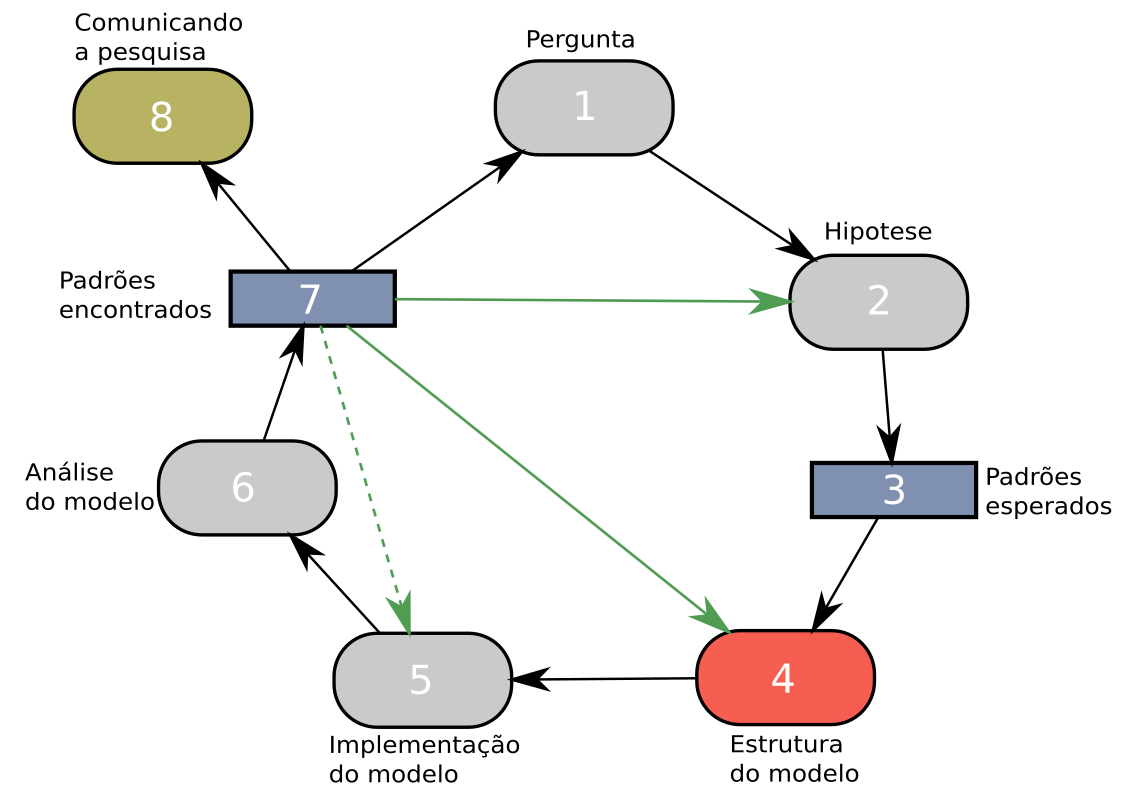
\includegraphics[height=.6\paperheight]{../Figures/intro/Ciclo_Grimm.png}
    \\{\footnotesize Fonte: Elaborada pelos autores}
    \label{fig:fluxoGrimm}
  \end{figure}

  

\end{frame}


\section{Fundamentação Teórica}


\begin{frame}{DFA - \cite{Peng_1994}}


  \begin{enumerate}
    \label{list:dfa}
    \item Pegando a série temporal \(\{x_{i}\}\) com  \(i\) variando de  \(1\) à \(N\), a série integrada \(X_{k}\) é calculada por \(X_{k} = \sum_{i=1}^{k}\left[x_{i} - \langle x \rangle \right] \) com \(k\) também variando entre \(1\) e \(N\);
    \item A série  \(X_{k}\) é dividida em \(N - n\) caixas de tamanho \(n\) (escala temporal), cada caixa contendo \(n + 1\) observações, iniciando em \(i\) até \(i + n\);
    \item Para cada caixa um polinômio (geralmente de grau 1) é ajustado, gerando \(\widetilde{X}_{k, i}\) com \( i \le k \le (i + n) \) eliminando assim a tendência (detrended values);
    \item  para cada caixa é calculado: \(f_{DFA}^{2}(n, i) = \frac{1}{1+n} \sum_{k=i}^{i + n}(X_{k}-\widetilde{X}_{k, i})^{2}\)
    \item Para todas as caixas de uma escala temporal o DFA é calculado como: \(F_{DFA}(n) = \sqrt{\frac{1}{N - n} \sum_{i=1}^{N-n} f_{DFA}^{2}(n, i)}\);
    \item Para um número de diferentes escalas temporais (n), com valores possíveis entre \( 4 \le n \le \frac{N}{4}\), a função \(F_{DFA}\) é calculada para encontrar a relação entre \(F_{DFA} \times n\)
  \end{enumerate}


\end{frame}

\begin{frame}
  \frametitle{DCCA - \cite{Podobnik2008}}
  \begin{enumerate}
    \label{list:dcca}
    \item Para duas séries temporais \(\{x_{i}\}\) e \(\{x_{i}\}\) com  \(i\) variando de  \(1\) à \(N\), as séries integradas \(X_{k}\) e \(Y_{k}\) são calculadas por \(X_{k} = \sum_{i=1}^{k}\left[x_{i} - \langle x \rangle \right] \) e \(Y_{k} = \sum_{i=1}^{k}\left[y_{i} - \langle x \rangle \right] \) com \(k\) também variando entre \(1\) e \(N\);
    \item As séries  \(X_{k}\) e \(X_{k}\) são divididas em \(N - n\) caixas de tamanho \(n\) (escala temporal), cada caixa contendo \(n + 1\) observações, iniciando em \(i\) até \(i + n\);
    \item Para cada caixa um polinômio (geralmente de grau 1) é ajustado, gerando \(\widetilde{X}_{k, i}\) para a primeira série e \(\widetilde{Y}_{k, i}\) para a segunda com \( i \le k \le (i + n) \) eliminando assim a tendência (detrended values);
    \item  Para cada caixa é calculado: $f_{DCCA}^{2}(n, i) = \frac{1}{1+n} \sum_{k=i}^{i + n}(X_{k}-\widetilde{X}_{k, i})(Y_{k}-\widetilde{Y}_{k, i})$
    \item Para todas as caixas de uma escala temporal a função $F_{DCCA}^{2}(n)$ é calculada por: $F_{DCCA}^{2}(n) = \frac{1}{N-n} \sum_{i=1}^{N-n} f_{DCCA}^{2}(n, i)$;
    \item Para um número de diferentes escalas temporais $(n)$, com valores possíveis entre \( 4 \le n \le \frac{N}{4}\), a função $F_{DCCA}^{2}(n)$ é calculada para encontrar a relação entre $F_{DCCA}^{2}(n) \times n$.
  \end{enumerate}
  
\end{frame}

\begin{frame}
  \frametitle{\pdcca - \cite{Zebende2011}}

  \begin{equation}
    \label{eq_pdcca}
    \rho DCCA(n) = \frac{F_{DCCA}^2 (n)}{ F_{DFA1} (n) F_{DFA2} (n)}
  \end{equation}

\end{frame}

\begin{frame}
  \frametitle{\dmc - \cite{Zebende2018}}
  \begin{equation}\label{eq:dmc}
  {DMC}_{x}^{2}  \equiv \rho_{y,x_{i}}(n)^{T} \rho^{-1}(n) \rho_{y,x_{i}}(n)
\end{equation}


\begin{equation}\label{eq:dmc_mat_inv}
  \rho^{-1}(n) = \left(\begin{matrix} 
    1 & \rho_{x_{1},x_{2}}(n)                       &  \rho_{x_{1},x_{3}}(n) & \dots  &  \rho_{x_{1},x_{i}}(n) \\
    \rho_{x_{2},x_{1}}(n) & 1                       &  \rho_{x_{2},x_{3}}(n) & \dots  &  \rho_{x_{2},x_{i}}(n) \\
    \vdots                &  \vdots                 &  \vdots                & \dots  & \vdots \\
    \rho_{x_{i},x_{1}}(n) & \rho_{x_{i},x_{2}}(n)   &  \rho_{x_{i},x_{3}}(n) & \dots  &  1 \\
    \end{matrix}\right)^{-1}
\end{equation}

  

\end{frame}

\begin{frame}
  \frametitle{Aprendizado de Maquina - Machine Learning}


  \begin{figure}[!htb]
    \centering
    \caption{Conceituação - AM}
    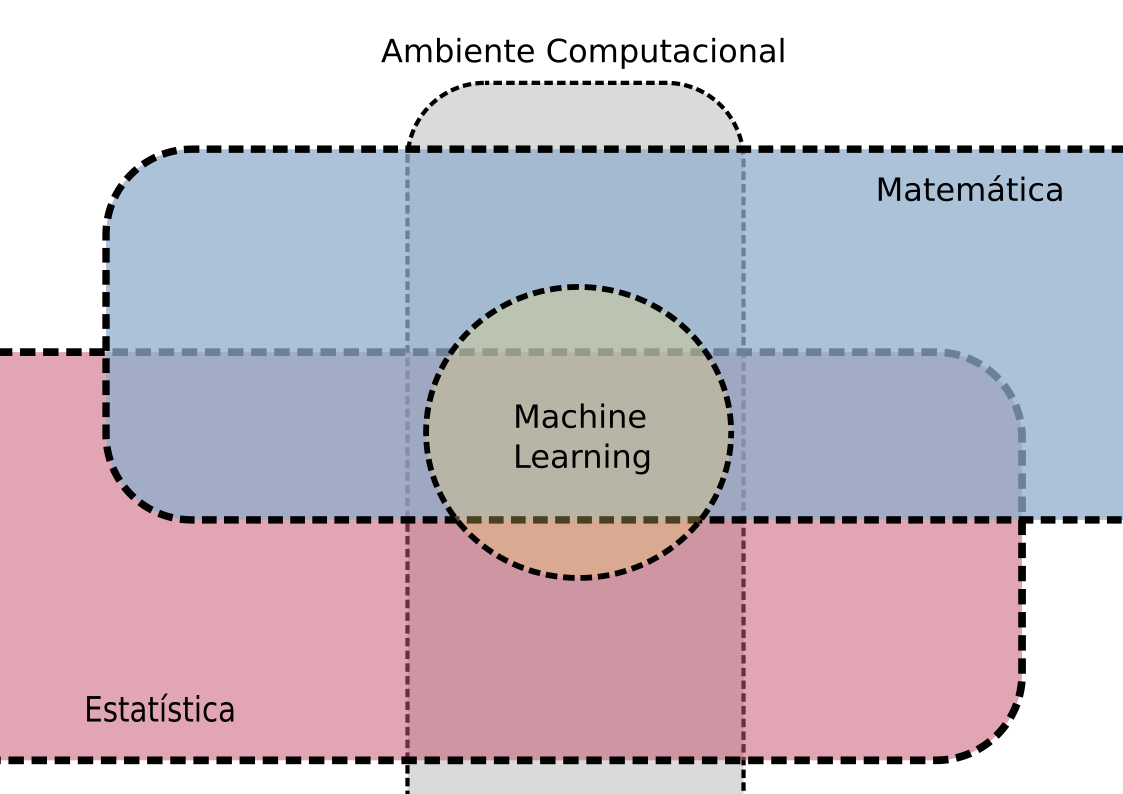
\includegraphics[height=.6\paperheight]{../Figures/ML/mat_est_ML.png}
    \\{\footnotesize Fonte: Elaborada pelos autores}
    \label{fig:diag_ml_01}
  \end{figure}

\end{frame}

\begin{frame}
  \frametitle{Aprendizado de Maquina - Machine Learning}

  \begin{figure}[!htb]
    \centering
    \caption{Diagrama conceitual - AM}
    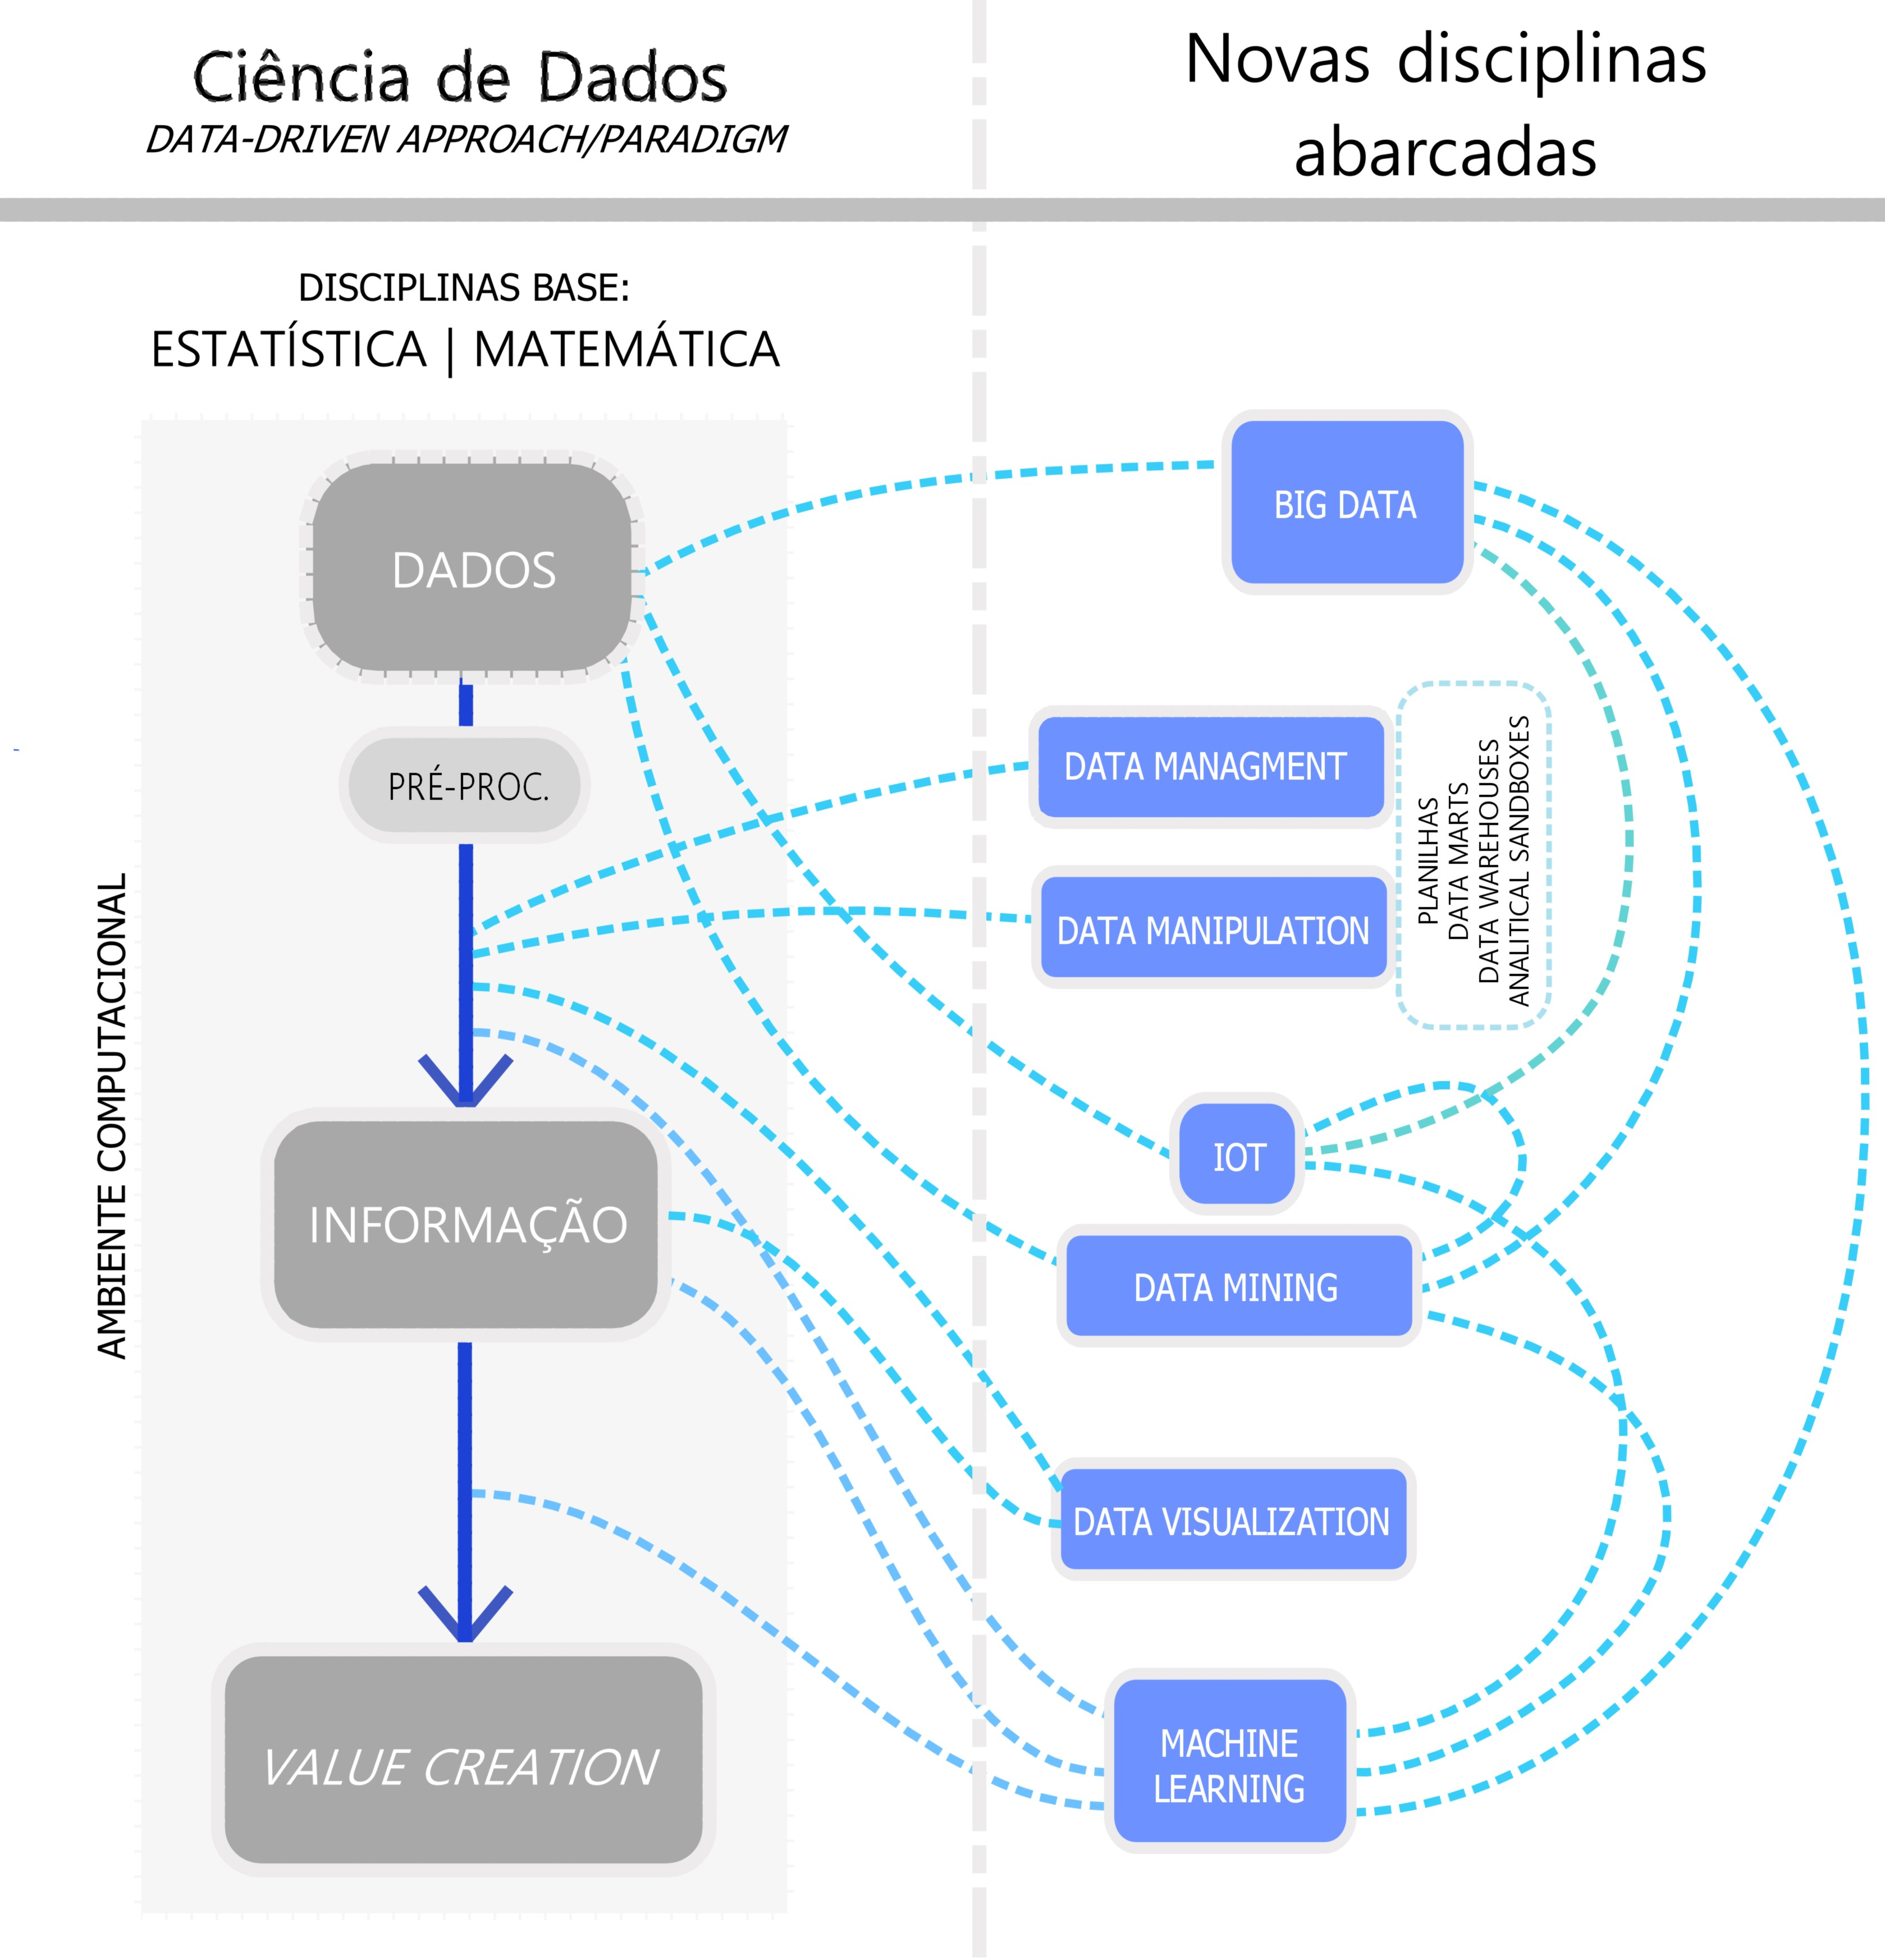
\includegraphics[height=.6\paperheight]{../Figures/ML/MAPA_conceitual_ciencia_de_dados_recorte.jpg}
    \\{\footnotesize Fonte: Elaborada pelos autores}
    \label{fig:diag_ml}
  \end{figure}

\end{frame}

\section{Resultados}

\begin{frame}{Produtos da Tese}
\begin{itemize}
	\item {Artigo: revisão de literatura.}
	\item Aplicativo de Cálculo do \dmc.
	\item Pacote Python para cálculo do DFA, DCCA, \pdcca, e  \dmc.
	\item Artigo: revista Software X.
	\item Artigo: análise de dados meteorológicos com \dmc

	\item Implementação do modelo de AM usando \dmc.
	\item Artigo: validação do modelo AM.
	\item Aplicação Artigo AM / dados meteorológicos
\end{itemize}

  
\end{frame}



\begin{frame}
  \frametitle{Artigo Publicado}

  \begin{figure}[!htb]
    \centering
    \caption{\cite{Oliveira2023}}
    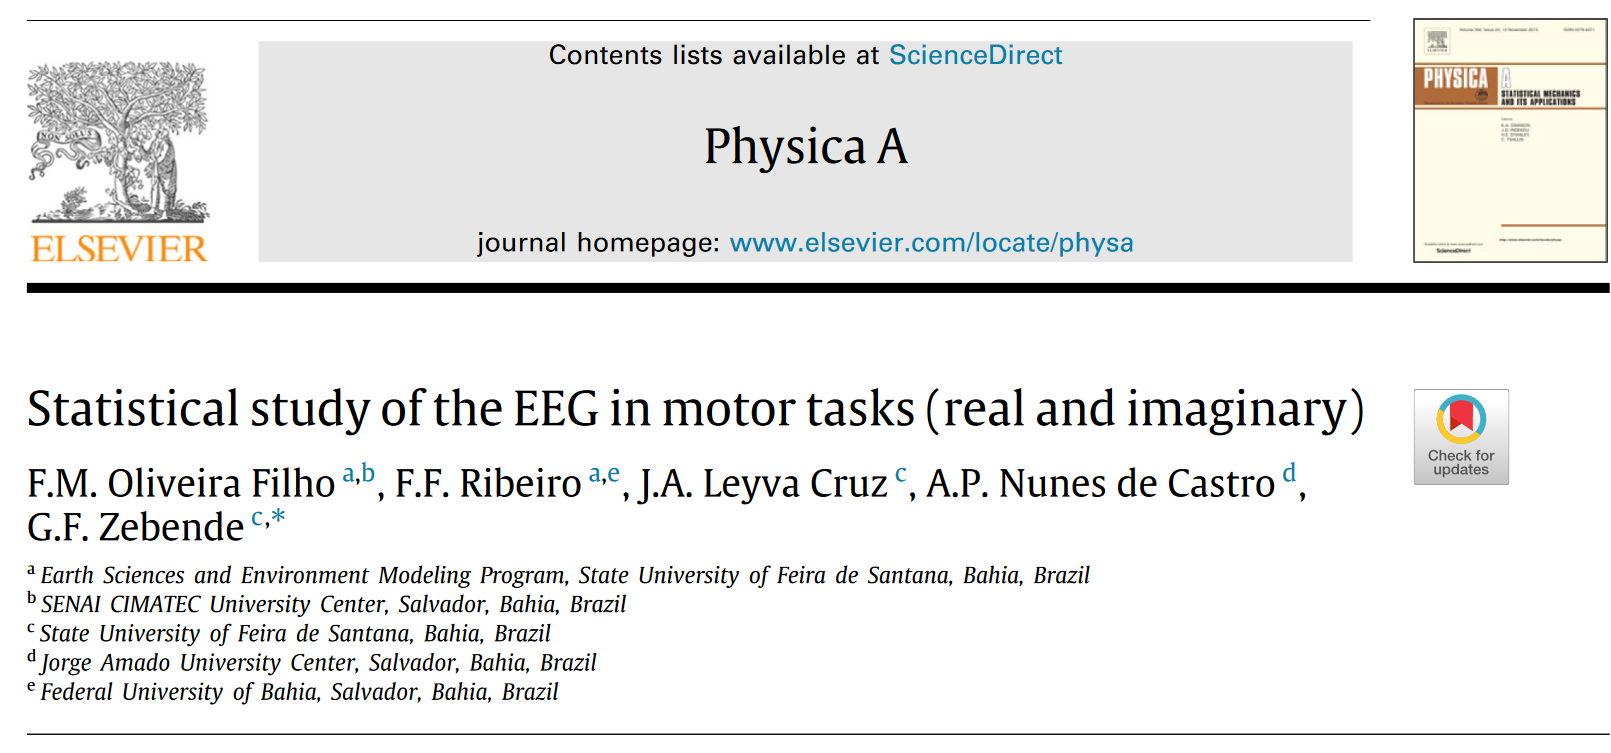
\includegraphics[height=.6\paperheight]{../Figures/artigos_publicados/artigo_01_abr_2023.png}
    \label{fig:ar_pub_01}
  \end{figure}

\end{frame}

% \section{Considerações Finais}

% \begin{frame}{Considerações Finais}



% \end{frame}


\section{Referências}

\begin{frame}[allowframebreaks]

  \bibliography{../References/referencias.bib}
  
\end{frame}

\section*{Obrigado}

\end{document}
